\chapter*{绪论}  % 第零章
\addcontentsline{toc}{chapter}{\protect\numberline{绪论}{}}

实变函数是为数学系本科高年级学生开设的一门重要的基础课程, 它是在实数理论和测度理论上建立起来的现代分析, 讲述了一般空间上测度论的基础知识和~$\mathbb{R}^n$~上的勒贝格积分理论, 为现代数学的许多分支如概率论、泛函分析、群上调和分析等提供了坚实的理论基础．

\section{黎曼积分理论的缺陷}

\subsection*{可积函数对连续性要求太强}

设~$f(x)$~为定义在区间~$[a,\,b]$~上的有界实值函数, 对~$[a,\,b]$~做分割
\[
a = x_0 < x_1 < \cdots < x_n = b
\]
称为~$[a,\,b]$~的一个划分. 记~$\lambda = \max \limits_{1 \leqslant i \leqslant n} |x_i - x_{i-1}|$.

对每个~$i=1,\,2,\,\cdots,\,n$, 令
\[
m_i = \inf \big\{f(x): \: x \in [x_{i-1},\,x_i]\big\}
\]
\[
M_i = \sup \big\{f(x): \: x \in [x_{i-1},\,x_i]\big\}
\]
则~$f(x)$~在~$[a,\,b]$~上黎曼可积的充要条件是
\begin{equation} \label{eq01}
\lim_{\lambda \to 0} \sum^n _{i=1} (M_i - m_i)(x_i - x_{i-1}) = 0
\end{equation}
其几何意义就是曲线~$y = f(x)$~的下方图形（曲边梯形）的外接阶梯形与内接阶梯形面积之差趋于零（图~\ref{fig01}）. 因此为保证~$f(x)$~在~$[a,\,b]$~上可积, $f(x)$~在~$[a,\,b]$~上的不连续点不能太多.

\begin{figure}[htbp]
\centering
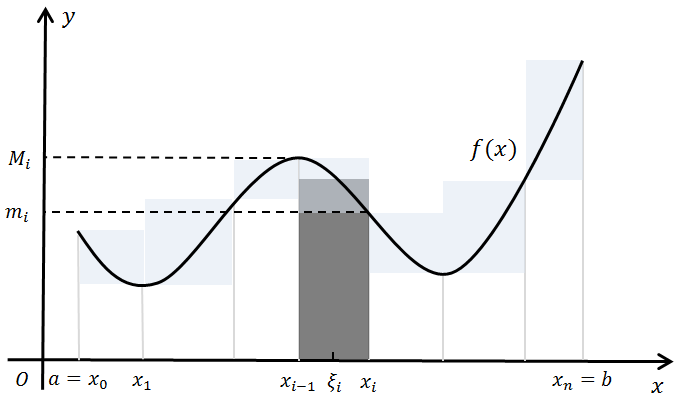
\includegraphics[width=0.7\textwidth]{image/Riemann.png}
\caption{黎曼可积的判别} \label{fig01}
\end{figure}

若条件~\eqref{eq01}~满足, 则~$f(x)$~在~$[a,\,b]$~上~的黎曼积分可表示为
\begin{equation} \label{eq02}
(R)\int_a ^b \!\! f(x) \mathrm{d}x = \lim_{\lambda \to 0} \sum^n _{i=1} f(\xi_i) \delta x_i
\end{equation}
其中, $\Delta x_i = x_i - x_{i-1}, \, \xi_i \in [x_{i-1},\,x_i]$. 注意, 这里的极限只是具有极限的形式, 不是一般意义上的极限.

由于黎曼积分对被积函数的连续性要求太强, 这样就限制了黎曼积分的应用.

例如, 狄利克雷函数
\[
D(x) = \left\{ \!\!
\begin{array}{ll}
1, & x \mbox{~为~} [0,\,1] \mbox{~上的有理数~} \\
0, & x \mbox{~为~} [0,\,1] \mbox{~上的无理数~}
\end{array}
\right.
\]
在~$[0,\,1]$~上不满足条件~\eqref{eq01}. 因此, $D(x)$~不是黎曼可积的.

\subsection*{积分与极限顺序不可交换}

设~$\{f_n(x)\}$~为~$[a,\,b]$~上的连续函数列, 且
\[
\lim_{n \to \infty} f_n(x) = f(x), \quad \forall~x \in [a,\,b]
\]
一般情况下, $f(x)$~在~$[a,\,b]$~上未必可积. 即使~$f(x)$~在~$[a,\,b]$~上可积, 也未必成立
\begin{equation} \label{eq03}
\lim_{n \to \infty} \int_a ^b \!\! f_n(x) \mathrm{d}x = \int_a ^b \!\! f(x) \mathrm{d}x
\end{equation}
为使~$f(x)$~在~$[a,\,b]$~上可积并且式~\eqref{eq03}~成立, 充分条件是~$\{f_n(x)\}$~在~$[a,\,b]$~上
一致收敛于~$f(x)$. 这不是必要条件（太强且不易验证）.

例如, 考虑~$[0,\,1]$~上的连续函数列~$f_n(x) = x^n, \, n = 1,\,2,\,\cdots$, 其极限为
\[
f(x) = \left\{ \!\!
\begin{array}{ll}
0, & x \in [0,\,1) \\
1, & x = 1
\end{array}
\right.
\]
易知, 式~\eqref{eq03}~成立, 但~$\{f_n(x)\}$~在~$[0,\,1]$~上不一致收敛于~$f(x)$
（因为连续函数列的一致收敛极限必连续, 而~$f(x)$~不连续）.

\subsection*{黎曼可积函数空间的不完备性}

$[a,\,b]$~上黎曼可积函数的全体构成的空间~$R[a,\,b]$~中, 并非每个柯西列都收敛, 即是不完备的.
而完备性在泛函分析理论中是非常重要的, 所以, $R[a,\,b]$~不是作为研究对象的理想空间.

以上几点表明, 黎曼积分有不少缺陷, 这就限制了黎曼积分的应用, 因此有必要加以改进.
20~世纪初, 法国数学家勒贝格~(1875\raisebox{0.5mm}{--}1941)~创建了一种新的勒贝格积分理论.
勒贝格积分理论是黎曼积分理论的推广和发展, 并且克服了黎曼积分理论的上述缺陷.

\section{勒贝格积分的大体思路}

为了使得很多连续性不好的函数也可积, 勒贝格提出了一种新的积分思想. 主要想法就是不从分割区间~$[a, \, b]$~着手,  而是从分割函数的值域出发.

为简单记, 这里只考虑~$f(x) \geqslant 0$~的情况. 注意到勒贝格积分的几何意义就是曲线~$y = f (x)$~的下方图形
~$G(f) = \big\{(x,\, y): \: a \leqslant x \leqslant b, \, 0 \leqslant y \leqslant f (x) \big\}$~的面积. 因此可以用下面的方式计算~$G(f)$~的面积.

令
\[
m = \inf \big\{f(x): \: x \in [a,\,b]\big\}, \quad M = \sup \big\{f(x): \: x \in [a,\,b]\big\}
\]
对~$[m,\,M]$~做分割
\[
m = y_0 < y_1 < \cdots < y_n = M
\]
记~$\lambda = \max \limits_{1 \leqslant i \leqslant n} |y_i - y_{i-1}|$. 令
\[
E_i = \big\{ x \in [a,\,b]: \: y_{i-1} \leqslant f(x) < y_i \big\}, \quad i = 1,\,2,\,\cdots,\,n
\]
则~$E_i$~是~$[a,\,b]$~的子集, 用~$|E_i|$~表示~$E_i$~的``长度''. 取~$\xi_i \in [y_{i-1},\,y_i]$, 则和式
\[
\sum^n _{i=1} \xi_i |E_i|
\]
是~$G(f)$~的近似值（图~\ref{fig02}）. 于是定义~$f(x)$~在~$[a,\,b]$~上的勒贝格积分为（若下面极限存在）
\begin{equation} \label{eq04}
(L)\int_a ^b \!\! f(x) \mathrm{d}x = \lim_{\lambda \to 0} \sum^n _{i=1} \xi_i |E_i|
\end{equation}

\begin{figure}[htbp]
\centering
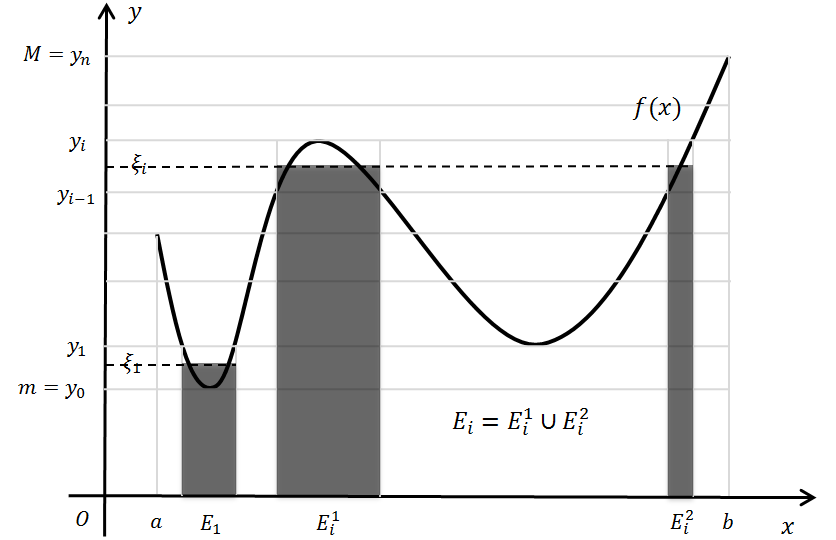
\includegraphics[width=0.8\textwidth]{image/Lebesgue.png}
\caption{勒贝格积分思想} \label{fig02}
\end{figure}

\begin{quote}
{\normalsize 对上述积分思想, 勒贝格自己曾作过一个比喻, 他说:
\begin{itemize}
  \item 假如我欠人家一笔钱, 现在要还, 此时按钞票的面值的大小分类, 然后计算每一类的面额总值, 再相加,
      这就是勒贝格积分思想;
  \item 如不按面额大小分类, 而是按从钱袋取出的先后次序来计算总数, 那就是黎曼积分思想.
\end{itemize}}
\end{quote}

按照勒贝格的方式定义积分的好处在于: 由于在每个~$E_i$~上, $f(x)$~的振幅都小于~$\lambda$,
因此很多连续性不好的函数也可积了. 但这产生了另一个困难: 要给出~$|E_i|$~的意义以及如何计算.

$|E_i|$~应该是一种类似区间长度的东西. 但是一般情况下, $E_i$~不是区间, 甚至也不是有限个不相
交区间的并, 因此必须对直线上比区间更一般的集合给出一种类似于区间长度的度量. 为
此, 勒贝格建立了测度理论, 并且在测度理论的基础上建立了勒贝格积分理论. 勒贝格 积分理论为建立近代分析理论打下了坚实的基础. 

\medskip

\section{本书的基本内容}

\qquad 本书的主要内容是紧紧围绕勒贝格积分理论的建立而展开的, 因此本书花了很大篇幅来介绍勒贝格测度理论.
由于测度理论要经常地遇到集合的运算和~$\mathbb{R}^n$~中的各种点集,  因此本书第一章先介绍了集合论和~$\mathbb{R}^n$~上点集的知识, 然后再介绍第二章勒贝格测度理论.

由于勒贝格测度理论并不能给直线上的每个集合定义测度, 只能对一部分集合即所谓``可测集''给出测度, 因此要定义~$f(x)$~的勒贝格积分, 必须要求由~$f(x)$~产生的形如
\[
E_i = \big\{ x: \: y_{i-1} \leqslant f(x) < y_i \big\}
\]
的集合是可测集, 这样的函数称为可测函数.

只有对可测函数才能定义新的积分, 因此在定义勒贝格积分之前, 需要定义可测函数并讨论可测
函数的性质, 这就是本书的第三章. 作了这些准备后, 就可以定义勒贝格积分,
并讨论勒贝格积分的性质以及与黎曼积分的关系, 构成本书的第四章.

进一步, 本书第五章利用勒贝格积分理论, 将黎曼积分的微积分学基本结果推广到更一般的函数类,
得到了勒贝格积分的微积分学基本定理、牛顿\raisebox{0.5mm}{--}莱布尼茨公式等, 使得勒贝格积分理论更加完善.

最后, 为了弥补黎曼可积函数空间不完备性缺陷, 本书在第六章介绍了所有~$p$~次幂~L-可积函数的全体构成
的空间\raisebox{0.5mm}{-----}$L^p$~空间理论, 讨论了勒贝格可积函数类的整体结构及其相互关系. $L^p$~空间的完备性和可分性为
人们解决一些具体数学问题带来了极大的便利, 为我们在其上建立分析学奠定了基础.
$L^p$~空间本身就是泛函分析课程中
巴拿赫空间的一类重要例子, 其理论也广泛地应用于微分方程、积分方程、傅里叶分析、有限元分析等许多领域.

